\documentclass[10pt,xcolor={usenames,dvipsnames}]{beamer}
\graphicspath{{pics/}}
\fontfamily{pnc}
\usepackage{verbatim}

\title{Final Presentation}
\subtitle{MyTaxiService}
\author{Roberto Clapis, Erica Stella}
\institute{Politecnico di Milano}
\date{12/02/2016}
\subject{Software Engineering 2}

\usepackage{graphicx}
\usebackgroundtemplate{
\includegraphics[width=\paperwidth,height=\paperheight]{background2.jpg}}

\setbeamercolor{frametitle}{fg=CornflowerBlue}
\setbeamercolor{title}{fg=CornflowerBlue}
\setbeamercolor{framesubtitle}{fg=RoyalBlue}

\addtobeamertemplate{frametitle}{\vskip+3ex}{}

\begin{document}
\frame{\titlepage}
\begin{frame}
	\frametitle{Table of Contents}
	\tableofcontents[currentsection]
\end{frame}


\section[Section]{RASD}

\begin{frame}
\begin{center}
	RASD	
\end{center}
\end{frame}
\begin{frame}
	\frametitle{The RASD Document}
	\framesubtitle{The approach}
	We tried to solve all the easy problems with a KISS approach, in order to focus on the actual difficulties. \\
	\begin{itemize}
		\item Login, logout, registration were kept as standard as possible
		\item Usability was kept in mind, customizability was not considered as a feature
		\item We tried to keep as little as possible the user inputs and let the application do the work
	\end{itemize}
\end{frame}

\begin{frame}
	\frametitle{Two simple interfaces}
	\framesubtitle{Adaptive web-based UI to ensure maintainability}
	\begin{center}
		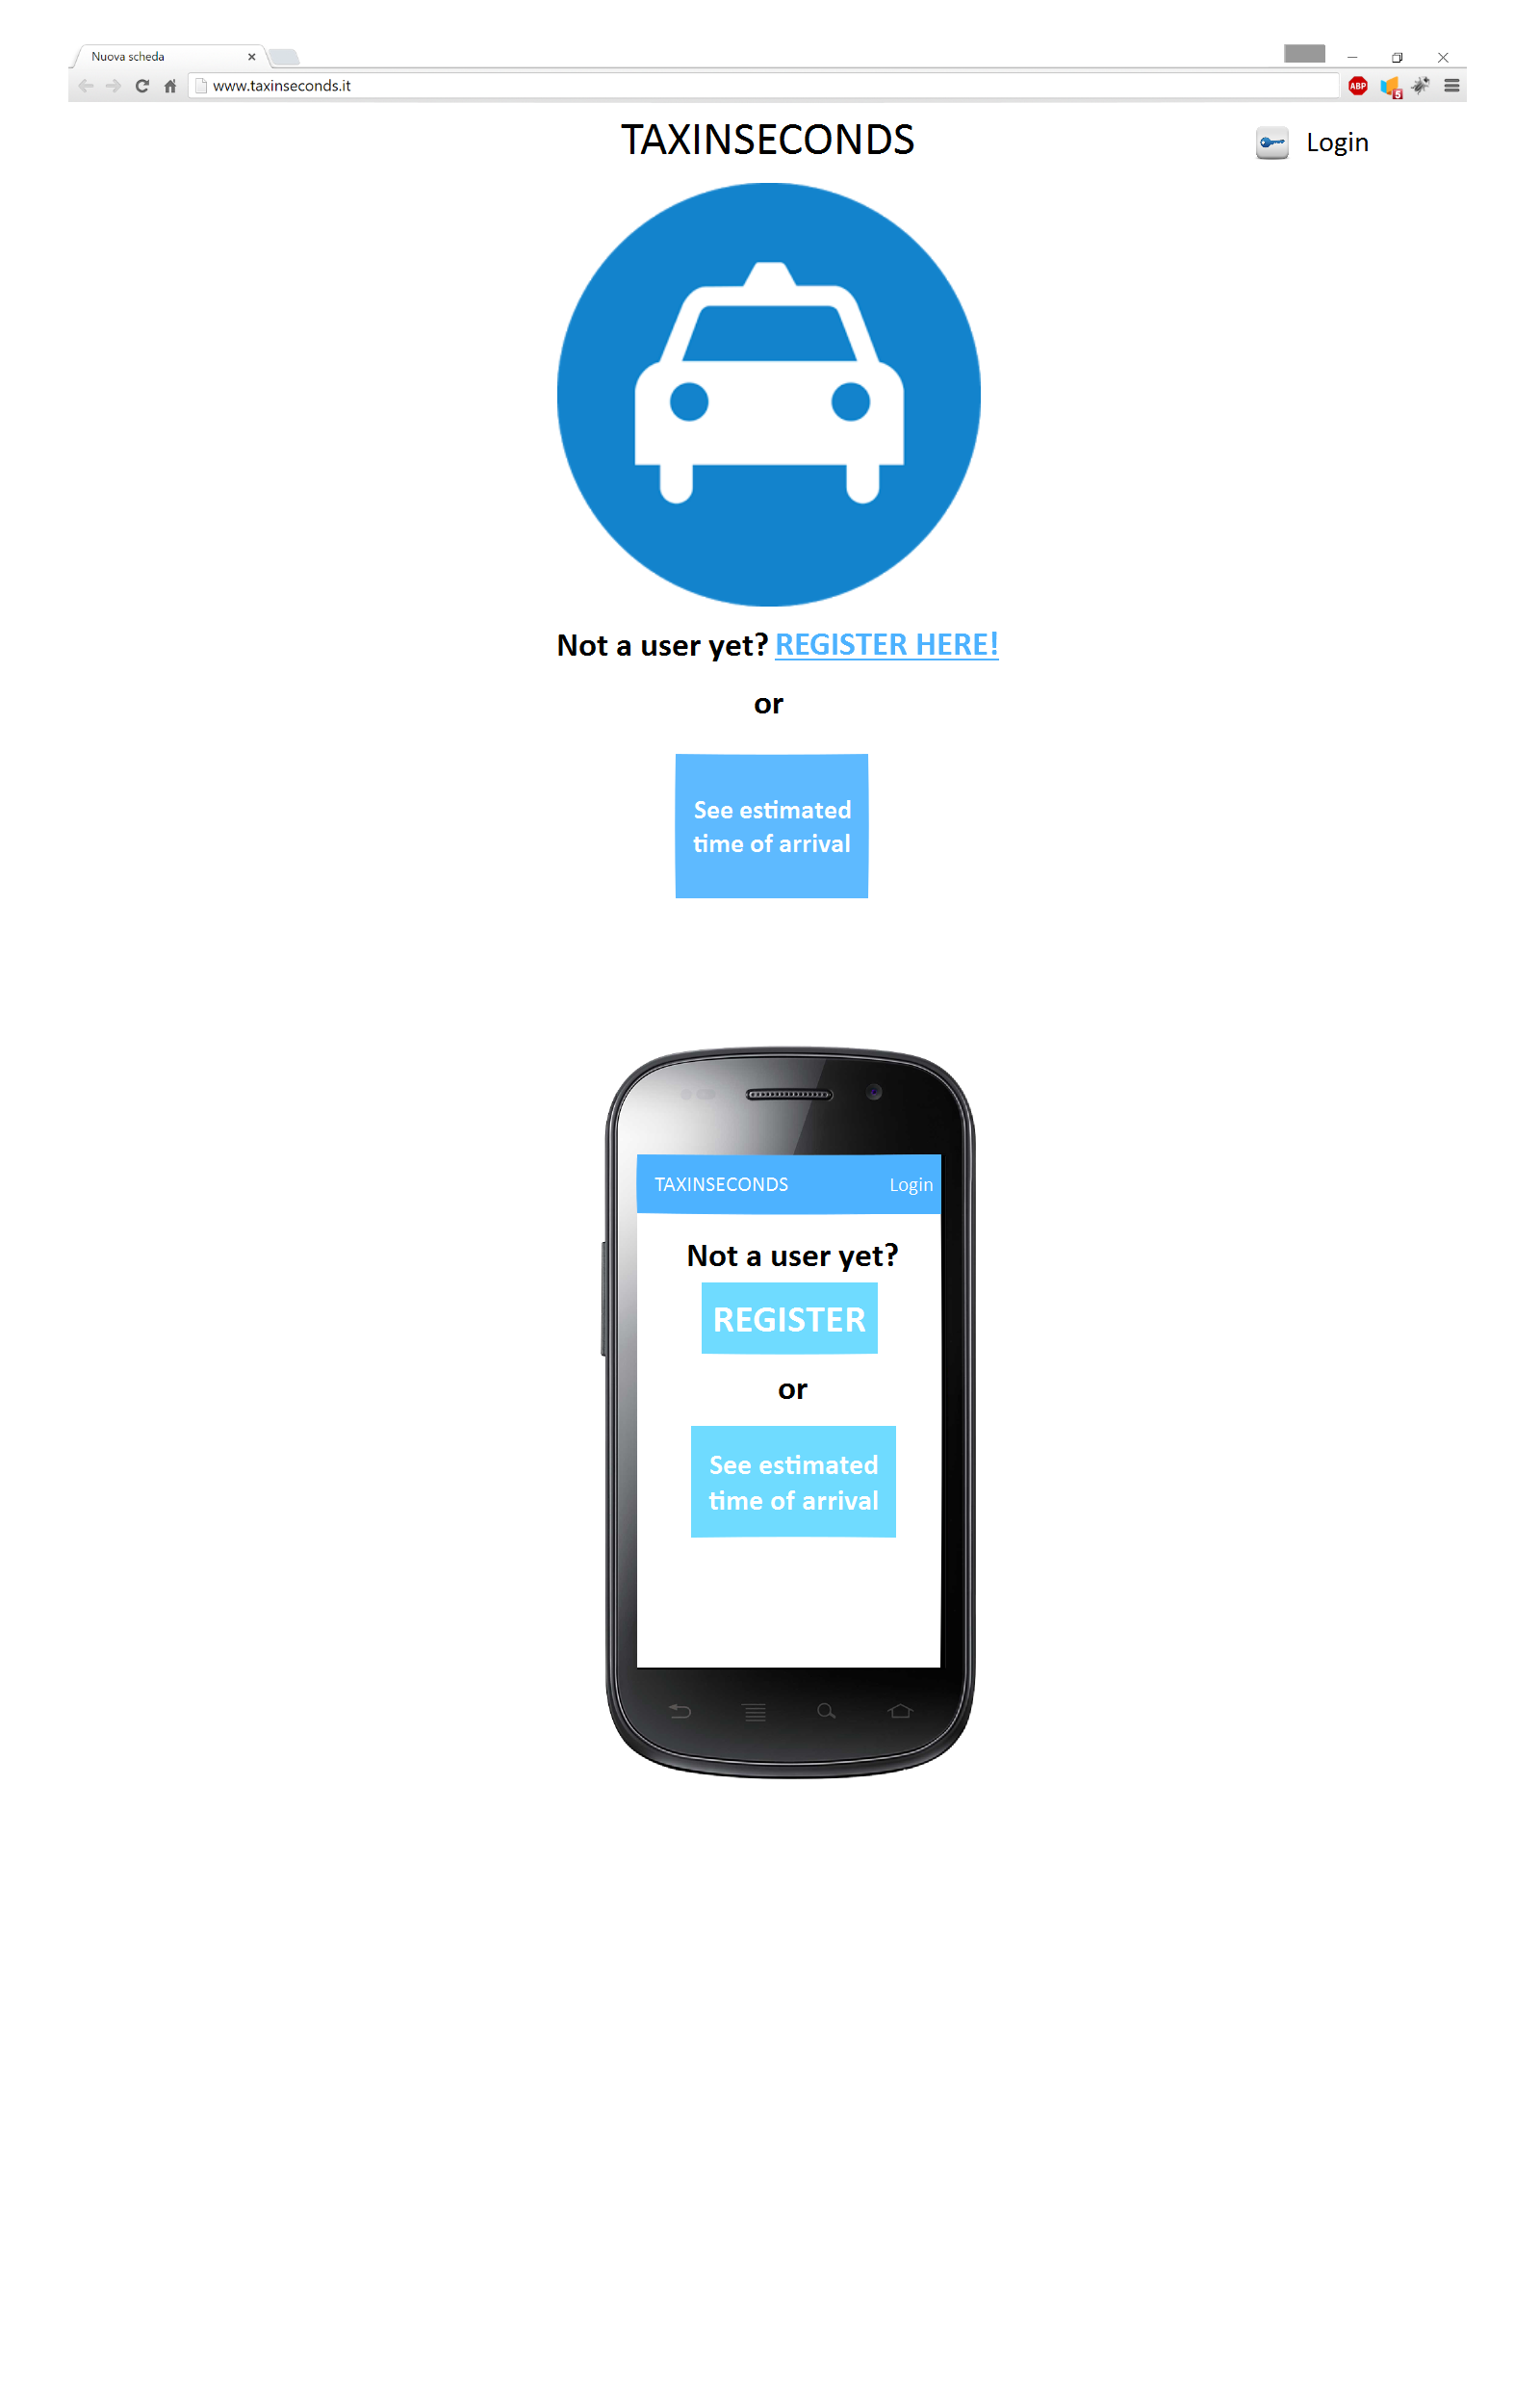
\includegraphics[width=\textwidth,height=\textheight,keepaspectratio]{GuestInterface}
	\end{center}
\end{frame}
\begin{frame}
	\frametitle{Use Cases}
	\framesubtitle{All the actions allowed were planned and analysed}
	\begin{center}
		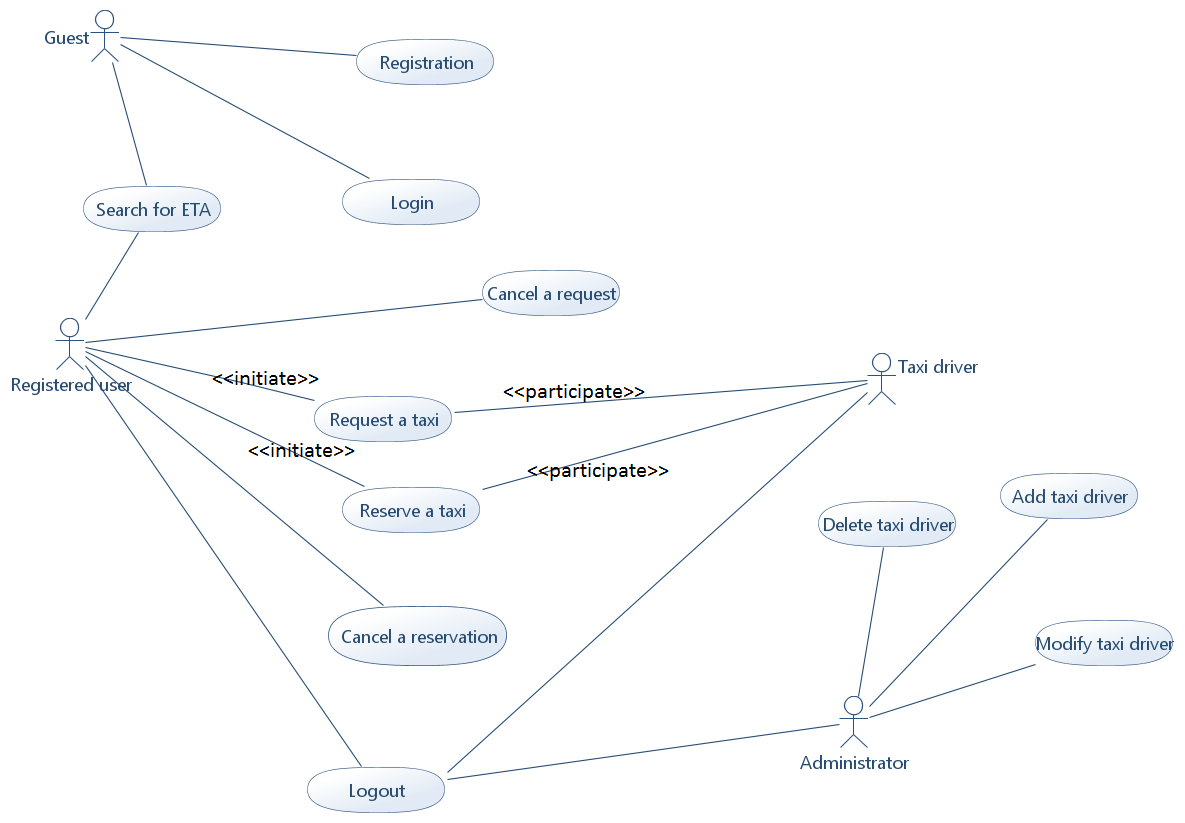
\includegraphics[width=\textwidth,height=\textheight,keepaspectratio]{UseCaseDiagram}
	\end{center}
\end{frame}
\begin{frame}
	\frametitle{Use Cases}
	\framesubtitle{Each use case is analysed in depth with a sequence diagram}
	\begin{center}
		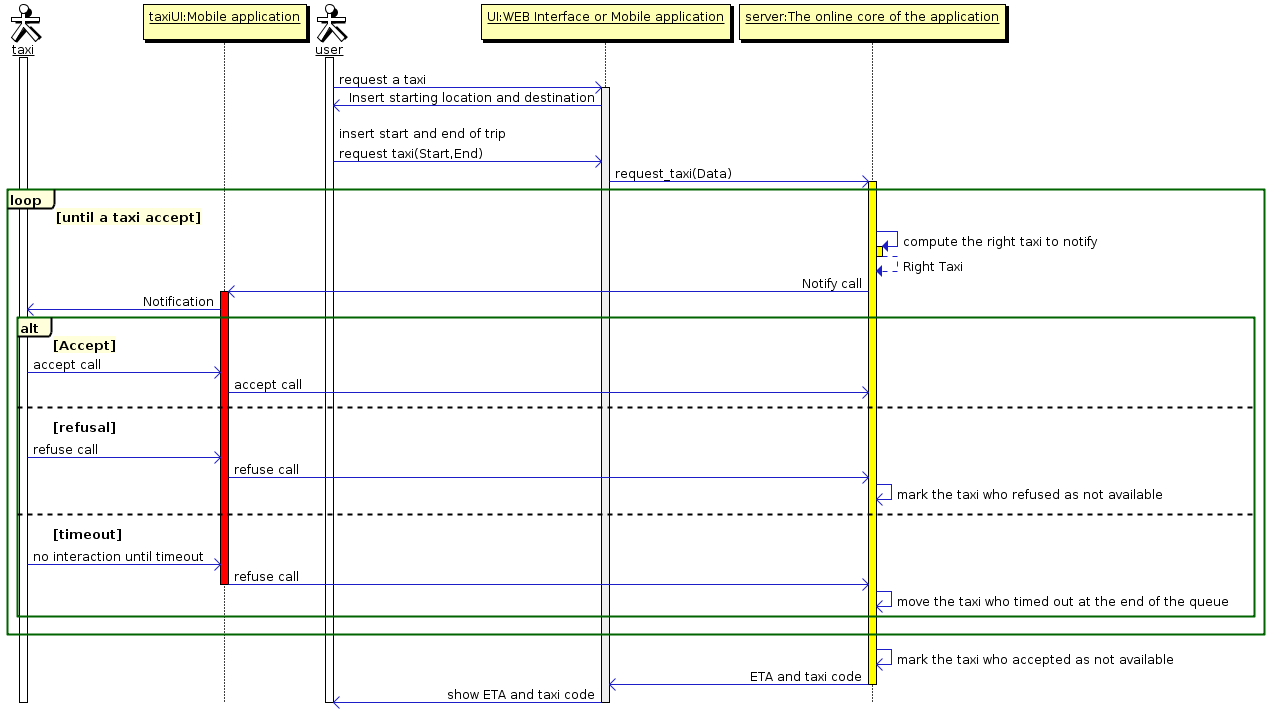
\includegraphics[width=\textwidth,height=\textheight,keepaspectratio]{request-a-taxi}
	\end{center}
\end{frame}
\begin{frame}
	\frametitle{Class Diagram}
	\framesubtitle{The class diagram was kept as readable as possible, underlying the main decisions taken}
	\begin{center}
		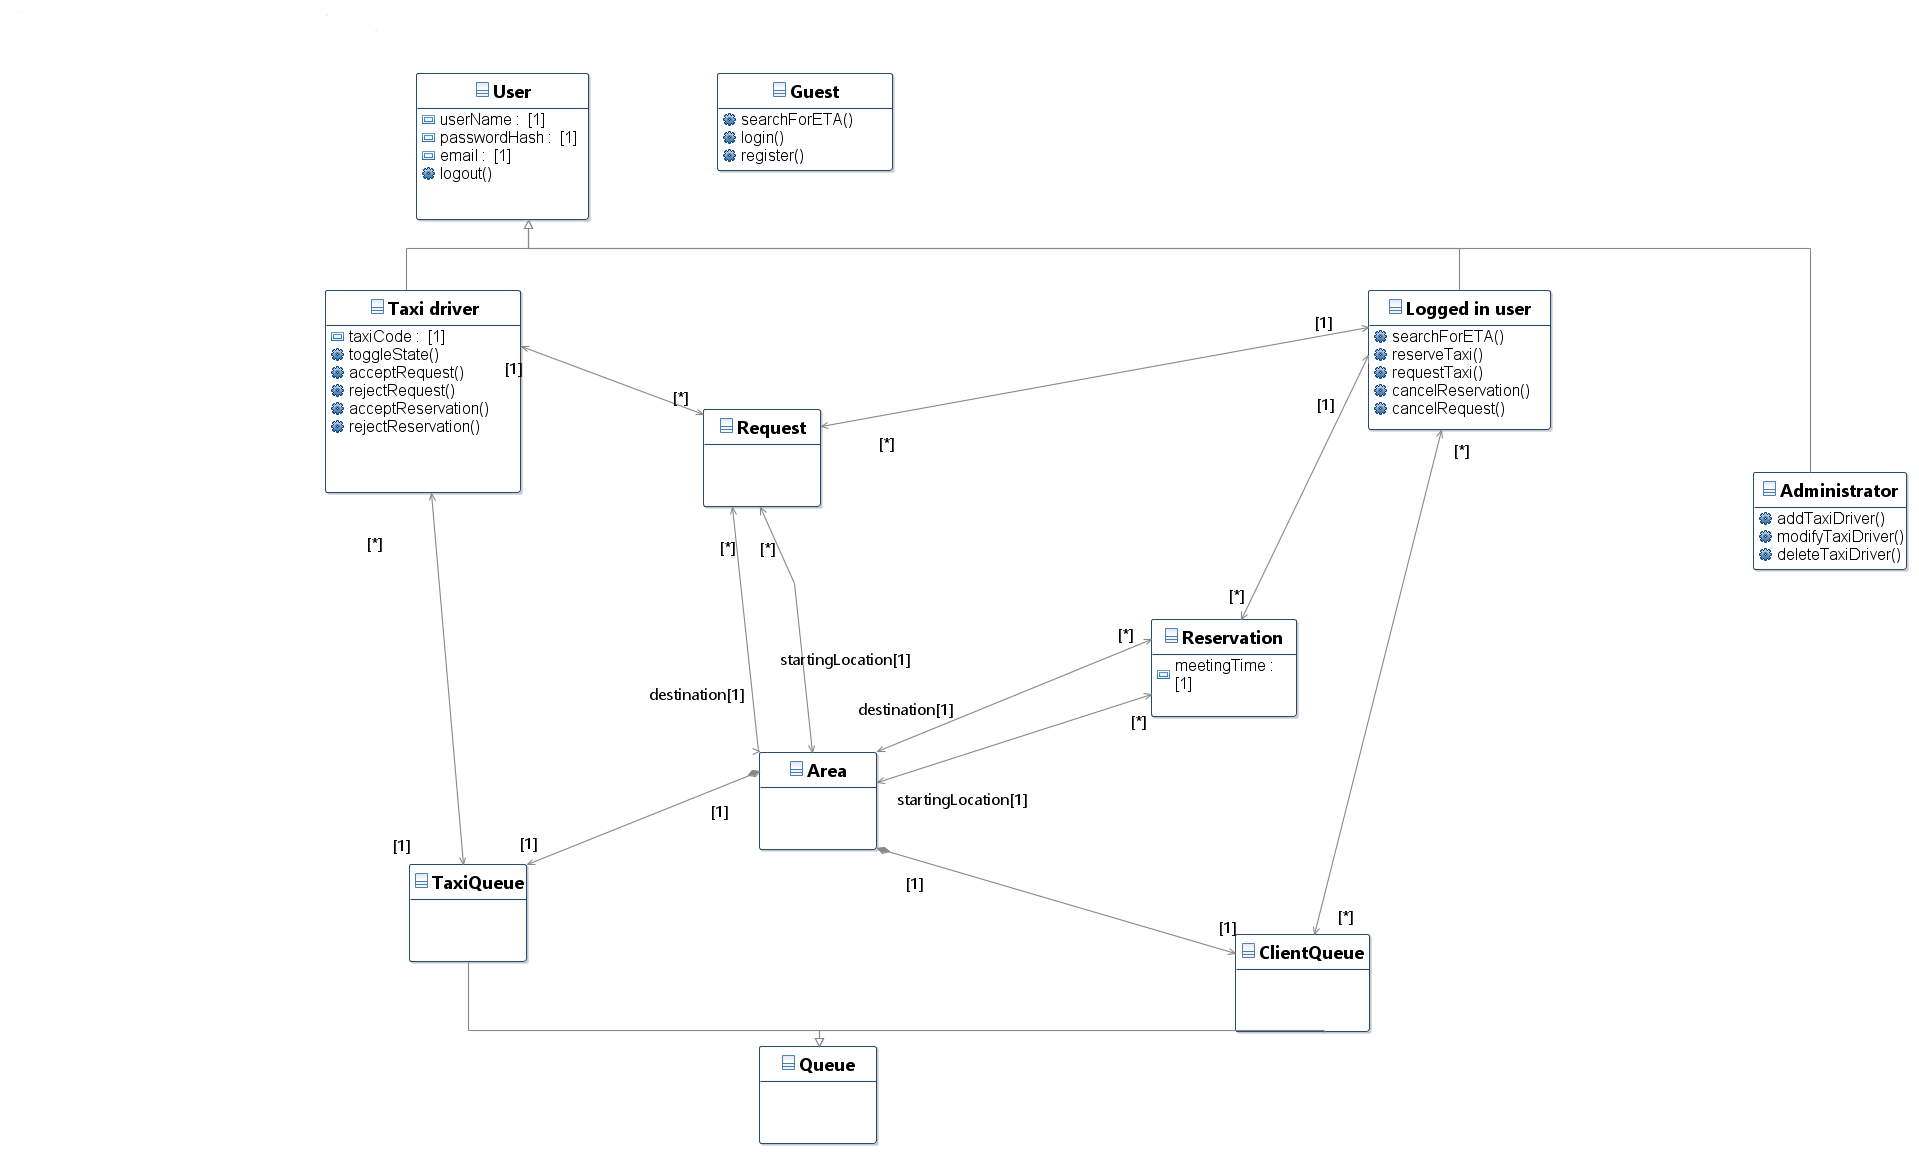
\includegraphics[width=\textwidth,height=\textheight,keepaspectratio]{ClassDiagram}
	\end{center}
\end{frame}
\begin{frame}
	\frametitle{Alloy}
	\begin{center}
		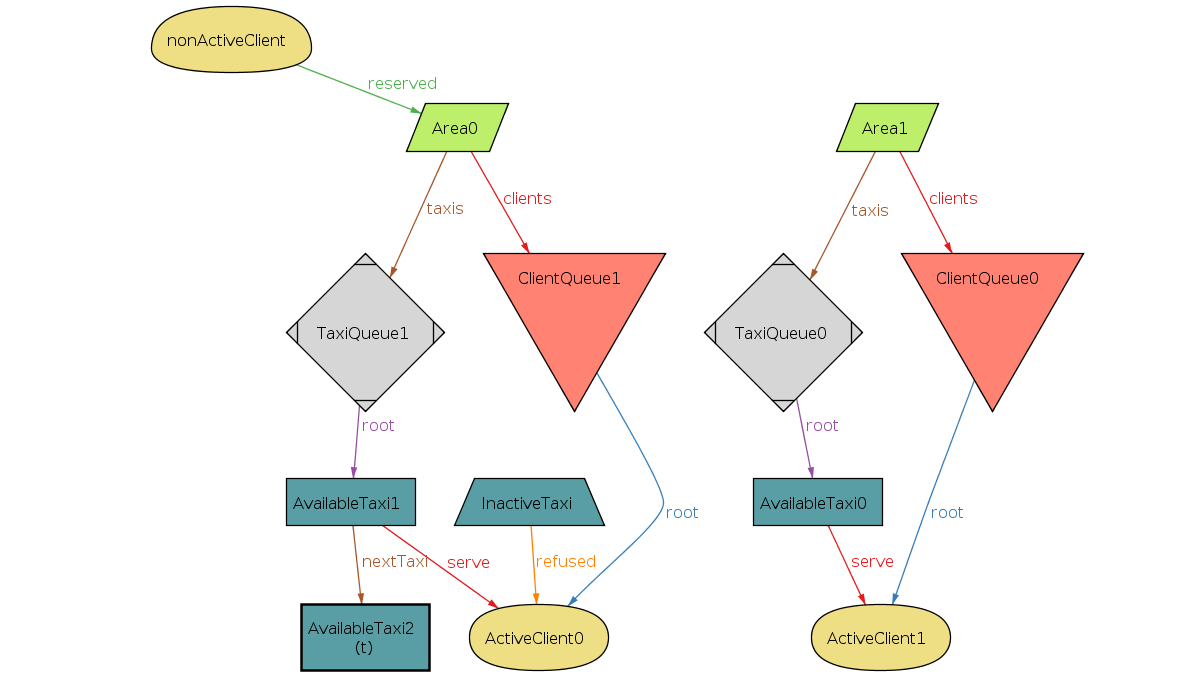
\includegraphics[width=\textwidth,height=\textheight,keepaspectratio]{reserved-and-refused}
	\end{center}
\end{frame}
\section[Section]{Design Document}
\begin{frame}
	\begin{center}
		Design Document
	\end{center}
\end{frame}
\begin{frame}
	\frametitle{}
	\framesubtitle{}
\end{frame}
\section[Section]{Test Document}
\section[Section]{Project Plan}
\section[Section]{Code Inspection}
\end{document}

\begin{frame}
	\frametitle{}
	\framesubtitle{}
\end{frame}
